\section{Auto-Triggering Function Generator}
\label{cp:AutoTriggeringFunctionGenerator}
Some applications require internal periodic or random triggering. The
\deviceName\ function generator provides this functionality.\par

The delay between two trigger pulses of this trigger generator is the sum of
two components: A fixed value $M$ and a pseudo-random value with a range given
by the exponent $N$. \par

The period is
\begin{align*}
    T = M + [1...2^N] - 1
\end{align*}
clock cycles\ 
\ifxHPTDC{%
    of the 150\,MHz.}
{
    \itett{
        with a duration of \SI{4}{\nano\second} per cycle for Gen\,1 and
        \SI{3.2}{\nano\second} for Gen\,2 \deviceName. The standard values of
        $M = 62500$ and $N = 0$ result in a frequency of \SI{4}{\kilo\hertz}
        for \deviceName\ Gen\,1 and \SI{5}{\kilo\hertz} for Gen\,2 devices.
    }{
        with a duration of \SI{4}{\nano\second} per cycle.
    }
}\par

The trigger can be used as a source for the TiGer unit (see
Section~\ref{cp:tiger}) \txh{and defines the period for the continuous mode
(see Section \ref{cp:continousmode})}{}{}.

\txh{
    \section{Continuous Mode\label{cp:continousmode}}
    This feature is only available for Gen\,2 devices of the \deviceName.\par

    The \deviceName\ continuously records stop signals even without a start
    signal connected. The data stream contains periodic packets with an
    absolute timestamp of 64 bits, followed by a list of stops relative to
    this timestamp.  The period of the timestamps can be adjusted using the
    Auto-Triggering Function Generator (see
    Section~\ref{cp:AutoTriggeringFunctionGenerator}) to adapt them to your
    evaluation interval.  Lower frequencies will create larger packets and
    have therefore a larger latency for receiving packets, potentially
    overflowing the buffers. Frequencies lower or equal to \SI{600}{\hertz}
    will contain rollover. Apart from that the choice is arbitrary.

    \section{Configurable Input Delay\label{cp:configurabledelay}}
    This feature is only available for Gen\,2 devices of the \deviceName.\par

    Each of the five input channels of the \deviceName\ can be delayed for up
    to \SI{204.6}{\nano\second} with a \SI{200}{\pico\second} granularity.
}{}{}

\section{Timing Generator (TiGer)\label{cp:tiger}}
Each digital LEMO-00 input can be used as an \ifxHPTDC{AC coupled}{LVCMOS}
trigger output. The TiGer functionality can be configured independently for
each connector. See Section~\ref{cp:tigerblock} for a full description of the
configuration options.
% 
%

Figure~\ref{fig:matrix} shows how the TiGer blocks are connected. They can be
triggered by an OR of an arbitrary combination of inputs, including the
auto-trigger \ifxHPTDC{and the ADC}{}. Each TiGer can drive its output to its
corresponding LEMO connector. This turns the connector into an output. 

\ifxHPTDC{
    The TiGer outputs are AC coupled to the connector. They can be operated in
    one of the following modes: \begin{description}[style=nextline]
    \item[\PREFIX TIGER\tu OFF]
        No signal is output to the connector. 
    \item[\PREFIX TIGER\tu OUTPUT]
        In this mode the connector is output only. Pulses are unipolar with
        \SI{2}{\volt} amplitude.  Connected hardware must not drive any
        signals to connectors used as outputs, as doing so could damage both
        the \deviceName\ and the external hardware.  We recommend to only use
        short pulses to avoid undesirable baseline shift due to the AC
        coupling, but the device does not pose any restrictions on the duty
        cycle.  This mode can be used as a clock output with a frequency of
        $75/N$\,MHz for integer $N$.
    \item[\PREFIX TIGER\tu BIDI]
        In this mode the TiGer creates unipolar pulses with 1~V amplitude. The
        connector can still be used as an input.  Use short pulses to keep the
        probability of collision and the effect on the baseline low.	
    \item[\PREFIX TIGER\tu BIPOLAR]
        In this mode the connector creates bipolar pulses with 1~V amplitude.
        The connector can still be used as an input.  Pulses have no effect on
        the baseline offset.  TiGer should be configured with $stop = start$
        for minimum width bipolar pulses of $2 \times
        6.\overline{6}$\,ns.  The maximum bipolar pulse width is
        \texttt{XHPTDC8\tu TIGER\tu MAX\tu BIPOLAR\tu PULSE\tu LENGTH = 15}.    
    \end{description}
}{
    The TiGer is DC coupled to the connector. Connected hardware must not
    drive any signals to connectors used as outputs, as doing so could damage
    both the \deviceName\ and the external hardware.  Pulses that are short
    enough for the input AC coupling are available as input signals to the
    \deviceName.  This can be used to measure exact time differences between
    the generated output signals and input signals on other channels. 
    \itett{
        When using one of the input channels as a source for the TiGer, the
        expected latency between signal input and TiGer output is roughly
        \SI{95}{\nano\second}.
    }{}
}
\begin{figure*}[ht]
    \centering
    \ifxHPTDC { 
        % this is an XCIrcuit drawing  convertex from postscript with 
        %ps2pdf.exe -dEPSCrop xhptdc8_trigger_matrix.ps 
        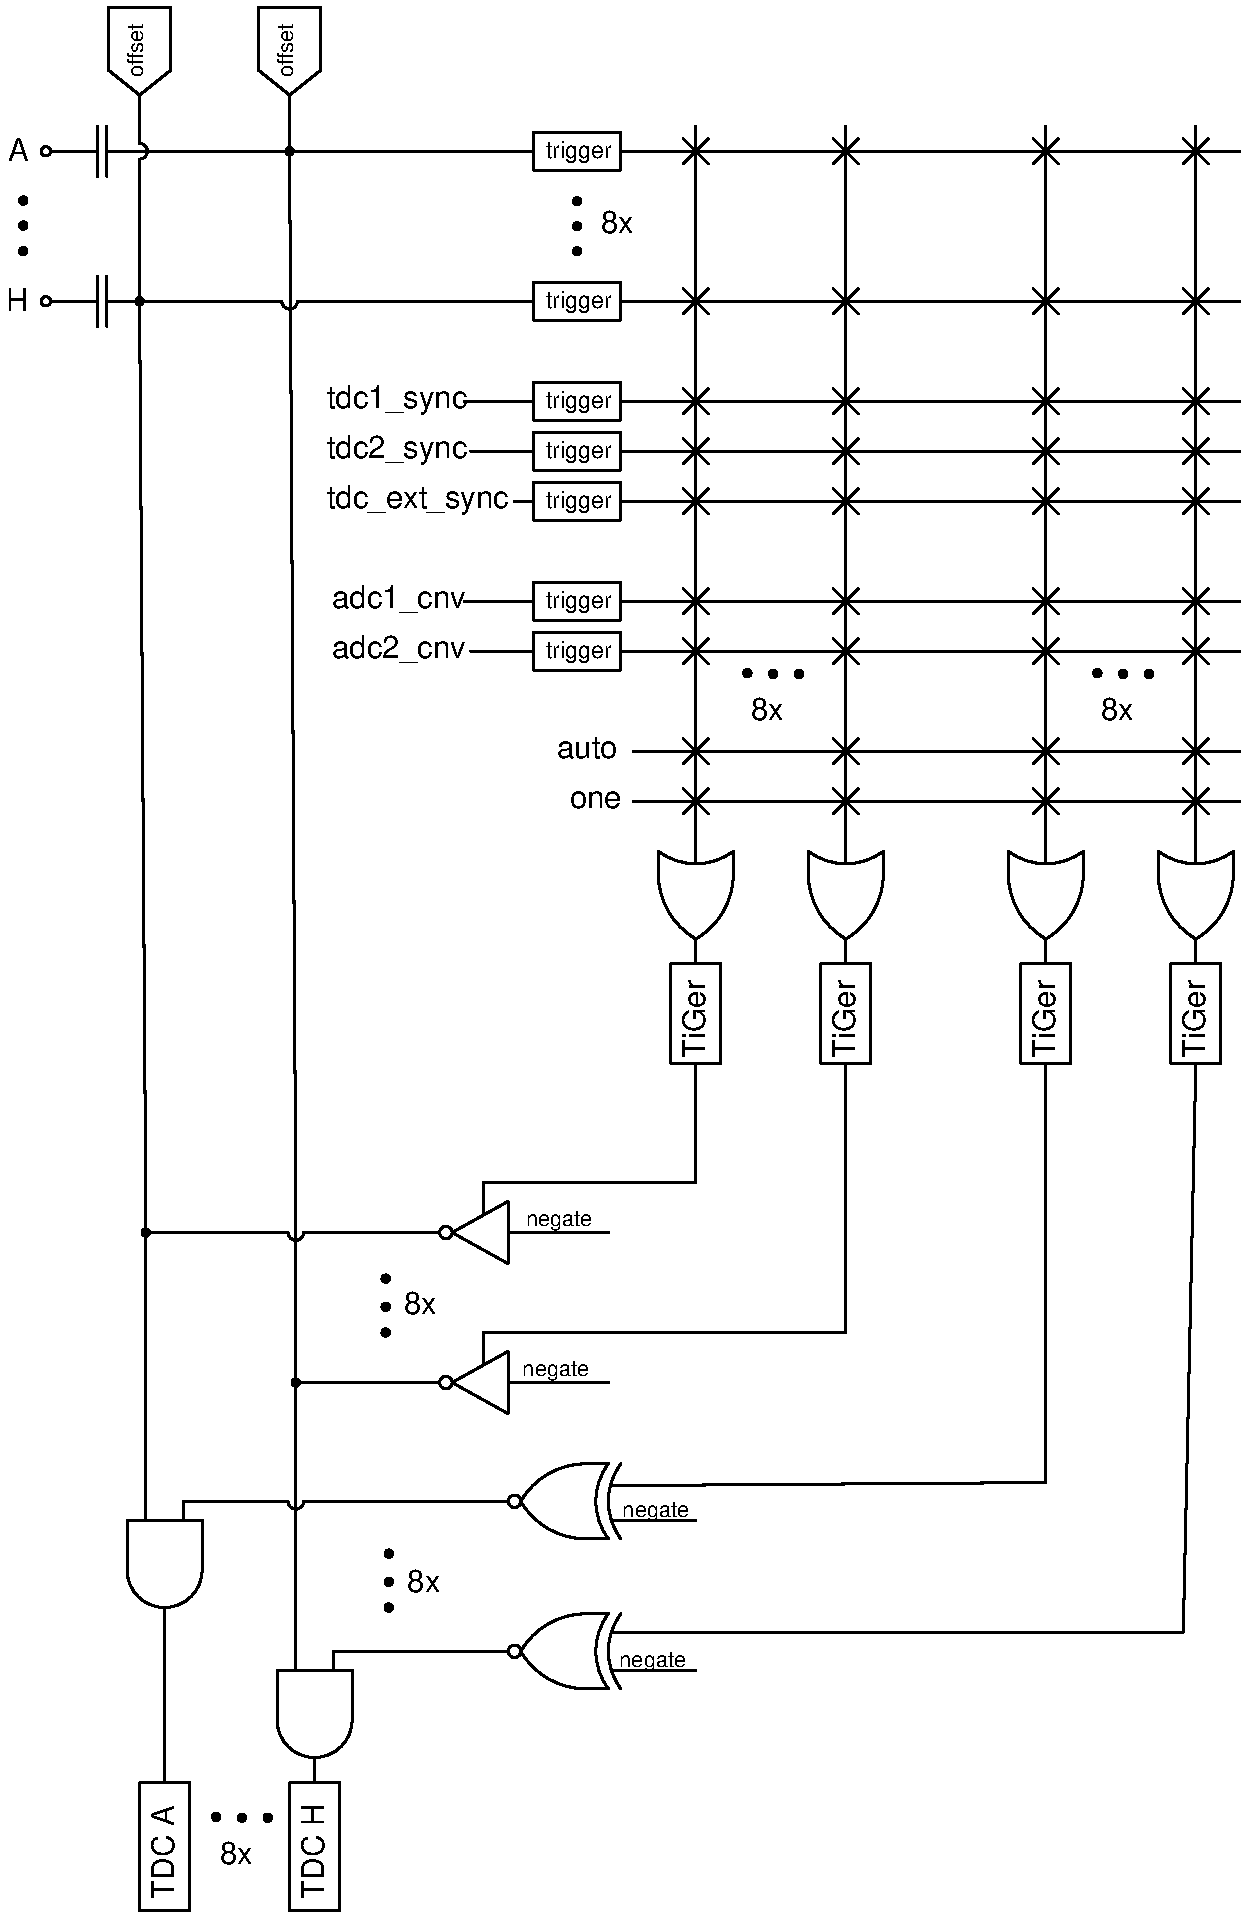
\includegraphics[width=0.6\textwidth]{
            xhptdc/figures/xhptdc8_trigger_matrix.pdf}
    }{ \includegraphics[width=\textwidth]{figures/xTDC4_tiger_matrix.pdf}
    }
    \caption{TiGer blocks can generate outputs that are also available on
        inputs.\label{fig:matrix}} 
\end{figure*}

\ifxHPTDC{
    \newpage
    \subsection{Trigger Sources}
    \label{triggersources}
    Trigger sources for TiGer and gating blocks are configured by a bit mask.
    You can combine any number of trigger source with a bit-wise OR.  The
    block will be trigger when any of the select trigger input is active. \begin{description}[style=nextline]
    \item[\PREFIX TRIGGER\tu SOURCE\tu NONE]
        Empty pattern that selects no trigger source.
    \item[\PREFIX TRIGGER\tu SOURCE\tu A to \tu H]
         TDC LEMO inputs.   
      \item[\PREFIX TRIGGER\tu SOURCE\tu TDC1\tu SYNC]
        Same as \texttt{\PREFIX TRIGGER\tu SOURCE\tu TDC2\tu SYNC}.\\
        Clock signal with $150/1024$\,\si{\mega\hertz}
        $\approx$ \SI{146.5}{\kilo\hertz}. 
    \item[\PREFIX TRIGGER\tu SOURCE\tu TDC\tu EXT\tu SYNC]
        Clock signal with \SI{125}{\kilo\hertz}. 
    \item[\PREFIX TRIGGER\tu SOURCE\tu AUTO]
        Periodic or random trigger pulses from the auto-trigger block.
    \item[\PREFIX TRIGGER\tu SOURCE\tu ADC1\tu CONV]
        Same as \texttt{\PREFIX TRIGGER\tu SOURCE\tu ADC2\tu CONV}. When there
        is an ADC trigger pulse on the TRG connector, either of the two
        onboard ADCs is triggered in an unpredictable pattern.  If the TRG
        input shall be used as a trigger, the trigger sources must contain
        both \texttt{ADC1\tu CNV} and \texttt{ADC2\tu CNV}.
    \item[\PREFIX TRIGGER\tu SOURCE\tu SOFTWARE]
        Set for one clock cycle by a call to the driver function
        \texttt{\prefix software\tu trigger()}.
    \item[\PREFIX TRIGGER\tu SOURCE\tu ONE]
        Trigger that is active on every clock cycle.
    \end{description}
    
    \ttinput{Tiger_Example.tex}	


    \subsection{Triggering the ADC with the TiGer}
    \label{adctiger}
    There is a ninth TiGer that is connected to the trigger input (TRG, see
    Figure~\ref{fig:bracket}) of the ADC. See Section~\ref{adc} for additional
    information on the ADC. 

    With retrigger enabled, the ADC TiGer can be used to periodically
    sample ADC data.  The period should be no shorter than
    \SI{300}{\nano\second} or 45 TiGer clocks.

    The ADC TiGer can also be used to sample voltages at a time relative
    to one of the TDC inputs. In this case, \texttt{stop} should be set to
    at least 45 to ensure that the sample period criterion is met even
    when pulses arrive in quick succession. A typical application would be
    to sample some slow control voltage once per start signal.

    \newpage
    \label{cp:gating}
    \section{Gating}
    Each TDC channel has a second, identical TiGer block that functions as a
    gate as shown in Figure~\ref{fig:matrix}. In the driver configuration
    structure (see Section~\ref{structchannel}), these are accessible as
    \mbox{\texttt{gating\tu block[channel]}}.  Hits are recorded in a channel
    only while the output of the gating block is active. Analogously, if the 
    gating block is negated in the configuration, hits are only recorded while
    the block is inactive.
    
    This is a useful feature in setups where the trigger creates a lot of
    noise.  A suitable configuration of the gating block can reduce the
    bandwidth and buffer usage significantly.  Gating is performed before the
    L0 buffer. Grouping is performed in software after readout. 

    Note that the gating logic is not instant but takes about six to seven
    clock cycles due to board-internal signal processing. 
    This means that there is a constant offset between the time an
    external trigger event is detected and the time the gating logic is
    enabled of up to about 50~ns.
    This offset does not exist if the (internal) auto-trigger functionality
    is utilized.

    When setting up the gating range, it is recommended to conservatively 
    choose the range (i.e., choose a bigger range than ultimately necessary).
    This is because at the edges of the gate, it is possible
    to create false timestamps due to how the gating logic is implemented: 
    The gate stores the state of the input channel from the last time the
    gate was active and updates the state once the gate is re-enabled. This
    update may be interpreted as an edge, at which point a timestamp is
    created that does not necessarily correspond to a real edge of an input
    signal (see also Figure~\ref{fig:gatingcaviat}).
    However, timestamps of signals that are not spanning over the edge of the 
    gate will always be correct.

    \begin{figure}[tbh]
        \centering 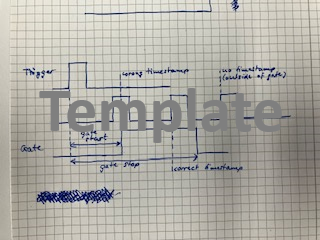
\includegraphics[width=0.6\linewidth]{figures/template.png}
        \caption{Example of a gating configuration. 
            At the edges of a gate, wrong timestamps may be created.
            The gate keeps the last state from when it was active (low signal
            level in the example) and updates it once it re-activates 
            (high signal level), which may be recorded as an edge.}
        \label{fig:gatingcaviat}
    \end{figure}

        
    \section{Triggerable ADC}
    \label{adc}
    The \deviceName\ is equipped with a triggerable ADC.  Whenever there is a
    rising edge on the ADC trigger connector (TRG, see
    Figure~\ref{fig:bracket}), the voltage on the ADC input connector is
    sampled. The result is inserted as a packet with a timestamp and an ADC
    value into the readout data stream. The timing resolution of the timestamp
	is 833\,ps.

    TRG is also connected to the output of a TiGer block.  This
    can be used  to trigger the ADC periodical or relative to one of the TDC
    inputs as described in Section~\ref{adctiger}

    The ADC triggers should be separated by at least 300\,ns.

    The width of the ADC input pulse should be larger than 13.2\,ns and
    smaller than 35\,ns.

    There are two interleaved ADCs to ensure that there is always an ADC
    available even during readout. This is exposed to the user both in the
    output data format and in the TiGer and Gating trigger sources.  When
    using the ADC trigger as a trigger for Gating or TiGer, both trigger
    sources shall be set to the same value.  During readout, the user shall
    not distinguish between data from the two ADCs unless advanced calibration
    is desired for the ADC data. In that case, the two ADCs should be treated
    separately.   
}{}